
\subsection*{Overall Performance}

The unregularized neural network archetecture (N) was not a top performer for any of the six datasets. 
At least one form of regularization outperformed the unregularized network for every dataset. 
No network with only a single form of regularization was a best-in-dataset performer, but networks 
with both dropout and weight decay were able to achive best-in-dataset performance on the Arabidopsis 
- Flowering and Wheat - Time Young Microspore genomic prediction tasks. These results are summarized 
in Table \ref{tab:model-comparison}.

These results support the hypothesis that some type of regularization is required to achieve
optimal performance in nerual network models. Additionally, a singular regularization strategy was
not optimal for all datasets, indicating that the best regularization strategy for genomic prediction
is dependent on the predicted species, trait, or population studied. 

Dropout regularization tends to produce networks 
that have reduced co-adaptation \citep{srivastava2014}. For genomic prediction tasks, this would
indicate that the detection of rare combinations haplotypes specific to only one
or two individuals are generally not learned or used for prediction. Instead, common haplotypes that persist across many
different dropout iterations would be preferred by the network during training.

Weight decay is an application of L2 regularization to neural networks \citep{krogh1992}. Like ridge regression, it prefers
solutions that do not place large emphasis on any singular feature. For genomic prediction tasks, 
this will produce models that perform well on traits with many predictive marker calls 
with small effects. 

For traits with a mixture of a few large-effect alleles and many small effect allels, some combination of 
L1 and L2 regularization may be optimal. The elastic net (EN) model incorporates both of these regularization
techniques, and is the top performer on two of the six datasets presented.


\ifdefined\showtablesandfigures
% Benchmark Datasets table.

\begin{table*}[htbp]
    \renewcommand{\familydefault}{\sfdefault}\normalfont
    \centering
    \caption{\bf Model Performance}

    \begin{tableminipage}{\textwidth}

        \begin{tabularx}{\textwidth}{ m{4.8em} m{4.8em} m{1.6em} m{1.6em} m{2.2em} m{1.6em} m{1.6em} m{1.6em} m{1.6em} m{1.6em} m{2.2em} }
\hline
\header & & \multicolumn{9}{c}{Accuracy} \\
\header & & OLS & RR & LASSO & EN & BRR & N & NWD & NDO & NWDDO \\
\hline
\header Species & Trait & & & & & & & & & \\
\hline
Arabidopsis & Dry Matter & 0.36 & 0.40 & 0.40 & \underline{0.42} & 0.39 & 0.38 & 0.35 & 0.39 & 0.40 \\
  & Flowering & 0.80 & 0.82 & 0.83 & 0.82 & 0.82 & 0.84 & 0.83 & 0.83 & \underline{0.86} \\
\hline
Maize & Flowering & 0.22 & 0.33 & 0.32 & 0.33 & 0.32 & 0.33 & 0.34 & \underline{0.35} & 0.33 \\
  & Grain Yield & 0.47 & \underline{0.59} & 0.49 & 0.51 & 0.57 & 0.55 & 0.52 & 0.55 & 0.51 \\
\hline
Wheat & Spike Grain Number & 0.15 & 0.27 & 0.33 & \underline{0.36} & 0.28 & 0.27 & 0.31 & 0.28 & 0.33 \\
  & Time Young Microspore & 0.59 & 0.61 & 0.74 & 0.73 & 0.64 & 0.67 & 0.74 & 0.68 & \underline{0.76} \\
\hline
\end{tabularx}

        \label{tab:model-comparison}
        \footnotesize  

        Accuracy of the best observed model performance on each dataset,
        rounded to three decimal places. The most accurate model on 
        each dataset is underlined for emphasis. 
        
    \end{tableminipage}
\end{table*}
 % Label = tab:model-comparison
\fi

\subsection*{Regularized Network Performance}

If a model is overfitted to training data, training data prediction accuracy is greater than 
the accuracy observed when making predictions on new datasets. Because all measurements were collected 
using five-fold cross validation sampling, models that overfit should exhibit lower accuracy. 
The decreased performance of the unregularized networks on several datasets in Figure 
\ref{fig-network-comparison} suggests that the overfitting problems 
previously observed were limiting out-of-sample performance. Our results demonstrate that 
applying one or more regularization methods to networks can improve their 
predictive accuracy for genomic prediction problems.

\ifdefined\showtablesandfigures

\begin{figure}[htbp]
\renewcommand{\familydefault}{\sfdefault}\normalfont
\centering 
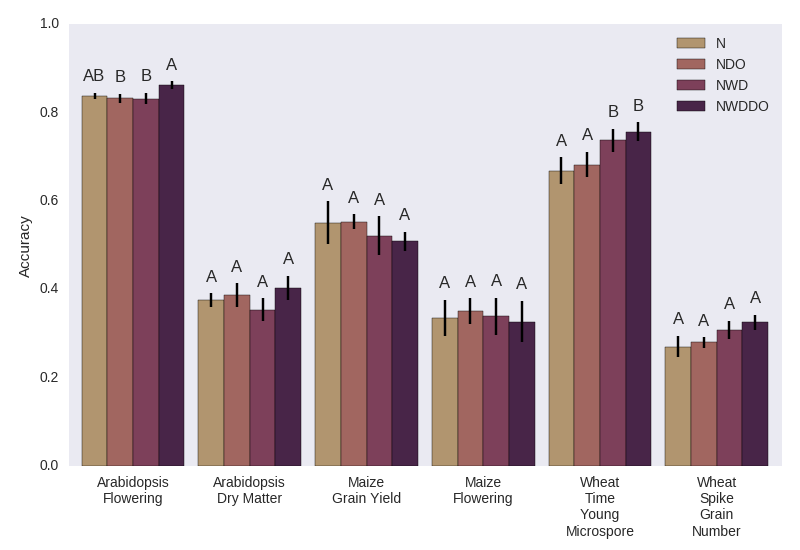
\includegraphics[width=\linewidth]{g3_article/figures/network_comparison.png}
    \caption{Predictive accuracy ($\mu \pm \sigma_{\bar{x}}$) of 
             regularized and non-regularized 
             neural network models for on benchmark datasets. Only the best performing
             network archetecture for each species, trait, and model is included. 
             The accuracy of the best performing model across all folds of data 
             and training cycles were recorded and compared. All pairwise model 
             comparisons within a species and trait were made using a two-sided paired t-test 
             (n=10, paired by training cycle and fold number).
             The resulting p-values were corrected for multiple comparisons within each 
             species and trait combination using the Holm-Bonferroni method. Columns annotated 
             with the same letter are not significantly different 
             at the $\alpha=0.05$ level.}
\label{fig:network-comparison}
\end{figure}
 % Label = fig:network-comparison
\fi

\subsection*{Deep Network Performance}

\ifdefined\showtablesandfigures

\begin{figure}[htbp]
\renewcommand{\familydefault}{\sfdefault}\normalfont
\centering 
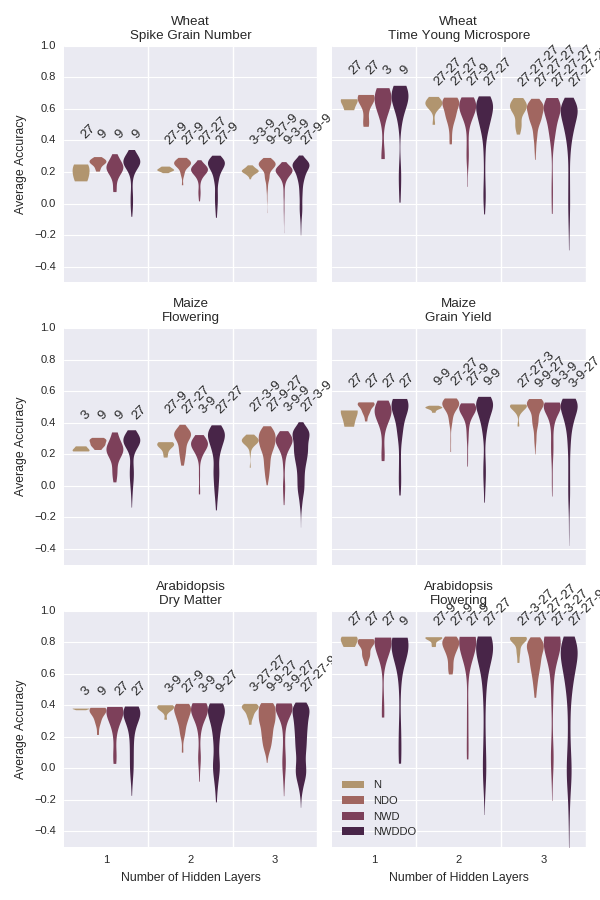
\includegraphics[keepaspectratio,height=\textheight,width=\linewidth]{g3_article/figures/depth_comparison.png}
    \caption{Distribution of predictive accuracy by benchmark dataset, network depth, 
             and model. The violin plot width indicates the Kernel Density Estimate 
             (KDE) of all observed accuracies of all models at a given network depth. 
             The sample size of the KDE is 7, 28, 28, and 112 samples for the 
             N, NWD, NDO, and NWDDO models, respectively. The models contributing 
             to each KDE vary across one or more of five weight decay, five dropout, 
             and seven hidden layer architecture parameters and can be 
             understood as the distribution of results across the set of 
             hyper-parameters to all network models with the same depth and regularization
             type. The KDE bandwidth parameters are set using Scott's normal reference rule. 
             The KDE plots are truncated to the minimum and maximum observed prediction accuracies.} 
\label{fig:depth-comparison}
\end{figure}

 % Label = fig:depth-comparison
\fi

\subsection*{GPU and CPU Training Time}

Network training time was significantly different from CPU training time in all datasets (Figure \ref{fig:time-comparison}).
For small networks trained on smaller datasets such as arabidopsis, CPU training completed significantly faster than GPU training, though only
by a small magnitude. For small networks and all other datasets, as well as for all large networks, GPU training time was faster than 
CPU training time on a per-core basis. For very large datasets such as the pig and loblolly datasets, CPU computing could not be 
completed in under 24 hours, but could be completed by a dedicated GPU card during that time. These results confirm that the 
speedups associated with GPU network training apply to genomic selection applications.  

The results from Figure \ref{fig:time-comparison} compare a single Intel i7-4790K CPU core to a single Nvidia GTX 680 graphics card.
However, most modern full-size computers posess multiple CPU cores, but few contain graphics cards with GPU compute capability. 
Thus, choosing a network training method depends on computing hardware availability as well as required turnaround time. Cloud providers such 
as Amazon Web Services (AWS) are becoming more popular, and make this choice somewhat less important. AWS provides both CPU and GPU rich 
machines which can be rented at low cost and are charged by the hour. This makes it feasible to choose a training platform 
that is most cost effective based on the quantity of data and desired network archetecture for any genomic selection application.

\ifdefined\showtablesandfigures

\begin{figure}[htbp]
\renewcommand{\familydefault}{\sfdefault}\normalfont
\centering 
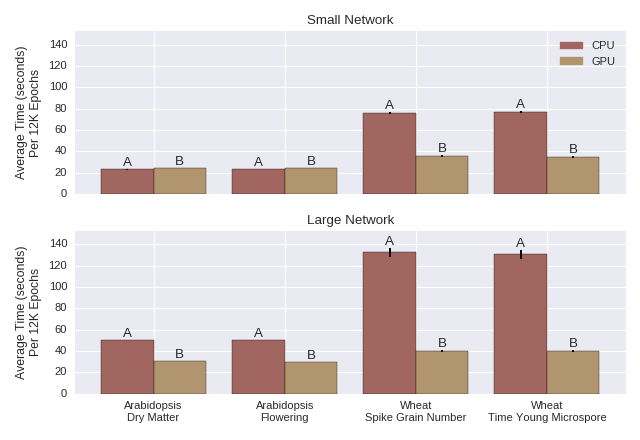
\includegraphics[keepaspectratio,width=\linewidth,height=\textheight]{g3_article/figures/time_comparison.png}
    \caption{Time to train different sized networks on identical datsets using a single dedicated CPU core
             compared to a single dedicated GPU card. Lower time to train is better. For the small network, 
             an unregularized, single hidden layer of 27 neurons was trained for 12K epochs on each dataset. 
             For the large network, two the hidden layers of size 64 and 32 neurons, respectively were trained. 
             Training processes were otherwise equal. This process was repeated ten times per dataset to 
             reduce variation associated with non-deterministic processor scheduling and varying computer system load.
             The ten CPU and GPU training samples were compared using an independent samples T-test with $n=30$. 
             CPU-GPU pairs annotated with the same letter are not significantly different 
             at the $\alpha=0.05$ level.}
\label{fig:time-comparison}
\end{figure}
 % Label = fig:time-comparison
\fi

%\section*{Additional guidelines}
%
%    \subsection*{Numbers} In the text, write out numbers nine or less except as part of a date, a fraction or decimal, 
%                          a percentage, or a unit of measurement. Use Arabic numbers for those larger than nine, 
%                          except as the first word of a sentence; however, try to avoid starting a sentence with such a number.
%
%    \subsection*{Units} Use abbreviations of the customary units of measurement only when they are preceded by a number: 
%            "3 min" but "several minutes". Write "percent" as one word, except when used with a number: 
%            "several percent" but "75\%." To indicate temperature in centigrade, use ° 
%            (for example, 37°); include a letter after the degree symbol only when some 
%            other scale is intended (for example, 45°K).
%
%    \subsection*{Nomenclature and Italicization} Italicize names of organisms even when  when the species is 
%        not indicated.  Italicize the first three letters of the names of restriction enzyme cleavage 
%        sites, as in HindIII. Write the names of strains in roman except when incorporating 
%        specific genotypic designations. Italicize genotype names and symbols, including all components 
%        of alleles, but not when the name of a gene is the same as the name of 
%        an enzyme. Do not use "+" to indicate wild type. Carefully distinguish between genotype 
%        (italicized) and phenotype (not italicized) in both the writing and the symbolism.
%
%\section*{In-text Citations}
%
%Add citations using the \verb|\citep{}| command, for example \citep{neher2013genealogies} or for multiple citations, \citep{neher2013genealogies, rodelsperger2014characterization}.
%
%For examples of different references, please see the example bibliography file 
%(accessible via the Project menu in the Overleaf editor). This contains examples 
%of articles \citep{neher2013genealogies, rodelsperger2014characterization}, a 
%book \citep{Sturtevent2001}, a book 
%chapter 
%XXXX-SKIPPED-XXXX
%%\citep{Sturtevent2001chp7}
%, ahead-of-print work \citep{Starita2015} and software \citep{Kruijer2015}.
%
%\section*{Examples of Article Components}
%\label{sec:examples}
%
%The sections below show examples of different header levels, which you can use in the primary sections of the manuscript (Results, Discussion, etc.) to organize your content.
%
%\section*{First level section header}
%
%Use this level to group two or more closely related headings in a long article.
%
%\subsection*{Second level section header}
%
%Second level section text.
%
%\subsubsection*{Third level section header:}
%
%Third level section text. These headings may be numbered, but only when the numbers must be cited in the text. 
%
%\section*{Figures and Tables}
%
%Figures and Tables should be labelled and referenced in the standard way using the \verb|\label{}| and \verb|\ref{}| commands.
%
%\subsection*{Sample Figure}
%
%Figure \ref{fig:spectrum} shows an example figure.
%
%\begin{figure}[htbp]
%\renewcommand{\familydefault}{\sfdefault}\normalfont
%\centering
%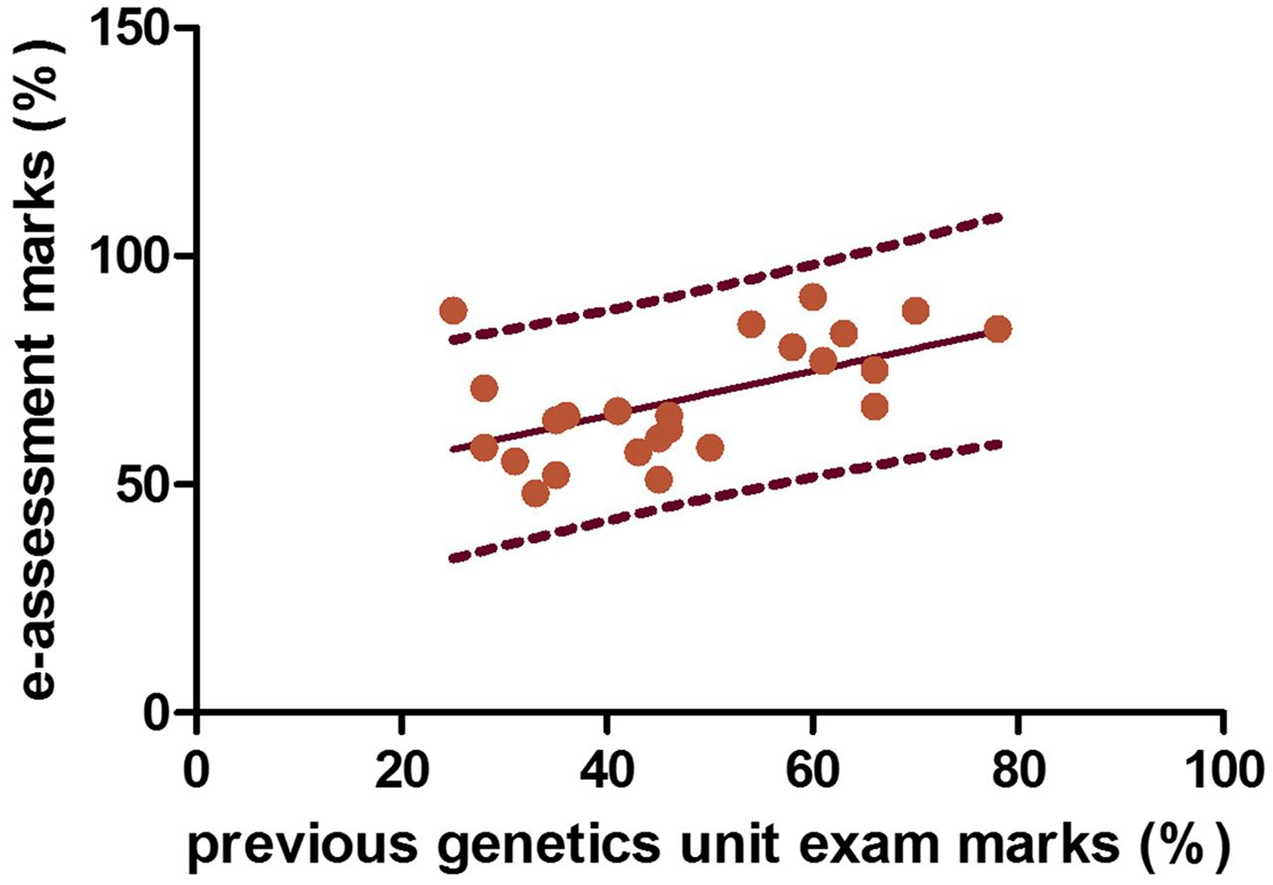
\includegraphics[width=\linewidth]{images/example-figure-g3}
%\caption{Example figure from \url{http://dx.doi.org/10.1534/g3.115.017509}. Please include your figures in the 
%    manuscript for the review process. You can upload figures to Overleaf via the Project menu. Upon acceptance, 
%    we'll ask for your figure files to be uploaded in any of the following formats: TIFF (.tiff), JPEG (.jpg), 
%    Microsoft PowerPoint (.ppt), EPS (.eps), or Adobe Illustrator (.ai).  Images should be a minimum of 
%    300 dpi in resolution and 500 dpi minimum if line art images.  RGB, CMYK, and Grayscale are all 
%    acceptable. Halftones should be high contrast with sharp detail, because some loss of detail and 
%    contrast is inevitable in the production process. Figures should be 10-20 cm in width and 1-25 cm 
%    in height. Graph axes must be exactly perpendicular and all lines of equal density.  Label 
%    multiple figure parts with A, B, etc. in bolded type, and use Arrows and numbers to draw attention 
%    to areas you want to highlight. Legends should start with a brief title and should be a 
%    self-contained description of the content of the figure that provides enough detail to fully 
%    understand the data presented. All conventional symbols used to indicate figure data points are 
%    available for typesetting; unconventional symbols should not be used. Italicize all mathematical 
%    variables (both in the figure legend and figure) , genotypes, and additional symbols that 
%    are normally italicized.  
%}%
%\label{fig:spectrum}
%\end{figure}
%
%\subsection*{Sample Video}
%
%Figure \ref{video:spectrum} shows how to include a video in your manuscript.
%
%\begin{figure}[htbp]
%\renewcommand{\familydefault}{\sfdefault}\normalfont
%\centering
%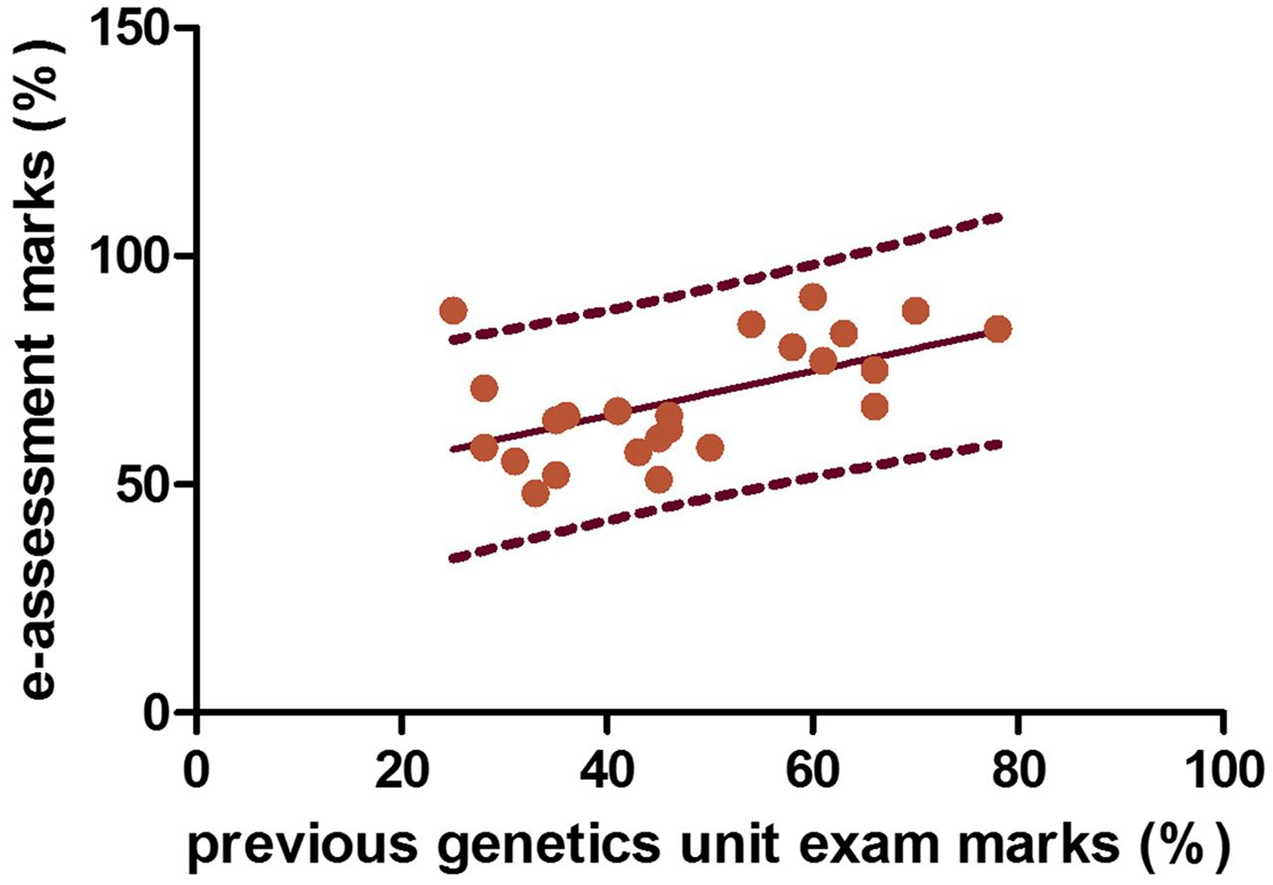
\includegraphics[width=\linewidth]{images/example-figure-g3}
%\caption{Example movie (the figure file above is used as a placeholder for this example). G3 supports video and movie 
%         files that can be linked from any portion of the article - including the abstract. Acceptable formats include 
%         .asf, avi, .wav, and all types of Windows Media files.   
%}%
%
%\label{video:spectrum}
%\end{figure}
%
%
%\subsection*{Sample Table}
%
%Table \ref{tab:shape-functions} shows an example table. Avoid shading, color type, line drawings, graphics, or 
%                                other illustrations within tables. Use tables for data only; present drawings, graphics, 
%                                and illustrations as separate figures. Histograms should not be used to present data 
%                                that can be captured easily in text or small tables, as they take up much more space.  
%
%Tables numbers are given in Arabic numerals. Tables should not be numbered 1A, 1B, etc., but if necessary, 
%interior parts of the table can be labeled A, B, etc. for easy reference in the text.  


%\begin{table*}[htbp]
%\renewcommand{\familydefault}{\sfdefault}\normalfont
%\centering
%\caption{\bf Students and their grades}
%\begin{tableminipage}{\textwidth}
%\begin{tabularx}{\textwidth}{XXXX}
%\hline
%\header Student & Grade\footnote{This is an example of a footnote in a table. Lowercase, superscript italic letters (a, b, c, etc.) are used by default. You can also use *, **, and *** to indicate conventional levels of statistical significance, explained below the table.} & Rank & Notes \\
%\hline
%Alice & 82\% & 1 & Performed very well.\\
%Bob & 65\% & 3 & Not up to his usual standard.\\
%Charlie & 73\% & 2 & A good attempt.\\
%\hline
%\end{tabularx}
%  \label{tab:shape-functions}
%\end{tableminipage}
%\end{table*}

%\section*{Sample Equation}
%
%Let $X_1, X_2, \ldots, X_n$ be a sequence of independent and identically distributed random variables with $\text{E}[X_i] = \mu$ and $\text{Var}[X_i] = \sigma^2 < \infty$, and let
%\begin{equation}
%S_n = \frac{X_1 + X_2 + \cdots + X_n}{n}
%      = \frac{1}{n}\sum_{i}^{n} X_i
%\label{eq:refname1}
%\end{equation}
%denote their mean. Then as $n$ approaches infinity, the random variables $\sqrt{n}(S_n - \mu)$ converge in distribution to a normal $\mathcal{N}(0, \sigma^2)$.
